\documentclass[twoside]{book}

% Packages required by doxygen
\usepackage{fixltx2e}
\usepackage{calc}
\usepackage{doxygen}
\usepackage[export]{adjustbox} % also loads graphicx
\usepackage{graphicx}
\usepackage[utf8]{inputenc}
\usepackage{makeidx}
\usepackage{multicol}
\usepackage{multirow}
\PassOptionsToPackage{warn}{textcomp}
\usepackage{textcomp}
\usepackage[nointegrals]{wasysym}
\usepackage[table]{xcolor}

% Font selection
\usepackage[T1]{fontenc}
\usepackage[scaled=.90]{helvet}
\usepackage{courier}
\usepackage{amssymb}
\usepackage{sectsty}
\renewcommand{\familydefault}{\sfdefault}
\allsectionsfont{%
  \fontseries{bc}\selectfont%
  \color{darkgray}%
}
\renewcommand{\DoxyLabelFont}{%
  \fontseries{bc}\selectfont%
  \color{darkgray}%
}
\newcommand{\+}{\discretionary{\mbox{\scriptsize$\hookleftarrow$}}{}{}}

% Page & text layout
\usepackage{geometry}
\geometry{%
  a4paper,%
  top=2.5cm,%
  bottom=2.5cm,%
  left=2.5cm,%
  right=2.5cm%
}
\tolerance=750
\hfuzz=15pt
\hbadness=750
\setlength{\emergencystretch}{15pt}
\setlength{\parindent}{0cm}
\setlength{\parskip}{3ex plus 2ex minus 2ex}
\makeatletter
\renewcommand{\paragraph}{%
  \@startsection{paragraph}{4}{0ex}{-1.0ex}{1.0ex}{%
    \normalfont\normalsize\bfseries\SS@parafont%
  }%
}
\renewcommand{\subparagraph}{%
  \@startsection{subparagraph}{5}{0ex}{-1.0ex}{1.0ex}{%
    \normalfont\normalsize\bfseries\SS@subparafont%
  }%
}
\makeatother

% Headers & footers
\usepackage{fancyhdr}
\pagestyle{fancyplain}
\fancyhead[LE]{\fancyplain{}{\bfseries\thepage}}
\fancyhead[CE]{\fancyplain{}{}}
\fancyhead[RE]{\fancyplain{}{\bfseries\leftmark}}
\fancyhead[LO]{\fancyplain{}{\bfseries\rightmark}}
\fancyhead[CO]{\fancyplain{}{}}
\fancyhead[RO]{\fancyplain{}{\bfseries\thepage}}
\fancyfoot[LE]{\fancyplain{}{}}
\fancyfoot[CE]{\fancyplain{}{}}
\fancyfoot[RE]{\fancyplain{}{\bfseries\scriptsize Generated by Doxygen }}
\fancyfoot[LO]{\fancyplain{}{\bfseries\scriptsize Generated by Doxygen }}
\fancyfoot[CO]{\fancyplain{}{}}
\fancyfoot[RO]{\fancyplain{}{}}
\renewcommand{\footrulewidth}{0.4pt}
\renewcommand{\chaptermark}[1]{%
  \markboth{#1}{}%
}
\renewcommand{\sectionmark}[1]{%
  \markright{\thesection\ #1}%
}

% Indices & bibliography
\usepackage{natbib}
\usepackage[titles]{tocloft}
\setcounter{tocdepth}{3}
\setcounter{secnumdepth}{5}
\makeindex

% Hyperlinks (required, but should be loaded last)
\usepackage{ifpdf}
\ifpdf
  \usepackage[pdftex,pagebackref=true]{hyperref}
\else
  \usepackage[ps2pdf,pagebackref=true]{hyperref}
\fi
\hypersetup{%
  colorlinks=true,%
  linkcolor=blue,%
  citecolor=blue,%
  unicode%
}

% Custom commands
\newcommand{\clearemptydoublepage}{%
  \newpage{\pagestyle{empty}\cleardoublepage}%
}

\usepackage{caption}
\captionsetup{labelsep=space,justification=centering,font={bf},singlelinecheck=off,skip=4pt,position=top}

%===== C O N T E N T S =====

\begin{document}

% Titlepage & ToC
\hypersetup{pageanchor=false,
             bookmarksnumbered=true,
             pdfencoding=unicode
            }
\pagenumbering{roman}
\begin{titlepage}
\vspace*{7cm}
\begin{center}%
{\Large My Project }\\
\vspace*{1cm}
{\large Generated by Doxygen 1.8.11}\\
\end{center}
\end{titlepage}
\clearemptydoublepage
\tableofcontents
\clearemptydoublepage
\pagenumbering{arabic}
\hypersetup{pageanchor=true}

%--- Begin generated contents ---
\chapter{Class Index}
\section{Class List}
Here are the classes, structs, unions and interfaces with brief descriptions\+:\begin{DoxyCompactList}
\item\contentsline{section}{\hyperlink{classCluster}{Cluster} \\*1 cluster contem 4 setores }{\pageref{classCluster}}{}
\item\contentsline{section}{\hyperlink{classCylinder}{Cylinder} }{\pageref{classCylinder}}{}
\item\contentsline{section}{\hyperlink{classFatEnt}{Fat\+Ent} }{\pageref{classFatEnt}}{}
\item\contentsline{section}{\hyperlink{classFatlist}{Fatlist} \\*Classe que vai ajudar a gravar o ultimo setor no disco }{\pageref{classFatlist}}{}
\item\contentsline{section}{\hyperlink{classFatTable}{Fat\+Table} }{\pageref{classFatTable}}{}
\item\contentsline{section}{\hyperlink{classHardDrive}{Hard\+Drive} }{\pageref{classHardDrive}}{}
\item\contentsline{section}{\hyperlink{classQtt}{Qtt} }{\pageref{classQtt}}{}
\item\contentsline{section}{\hyperlink{classSector}{Sector} \\*Unidades basicas de armazenamento (num HD orientado a setores) }{\pageref{classSector}}{}
\item\contentsline{section}{\hyperlink{classTime}{Time} \\*Final das Estruturas basicas }{\pageref{classTime}}{}
\item\contentsline{section}{\hyperlink{classTrack}{Track} }{\pageref{classTrack}}{}
\end{DoxyCompactList}

\chapter{Class Documentation}
\hypertarget{classCluster}{}\section{Cluster Class Reference}
\label{classCluster}\index{Cluster@{Cluster}}


1 cluster contem 4 setores.  




{\ttfamily \#include $<$estruturas.\+hpp$>$}

\subsection*{Public Member Functions}
\begin{DoxyCompactItemize}
\item 
\hyperlink{classSector}{Sector} {\bfseries g\+\_\+sector} (const ui \&i) const \hypertarget{classCluster_a26a447ffce23a83058de596992e037fa}{}\label{classCluster_a26a447ffce23a83058de596992e037fa}

\item 
vector$<$ \hyperlink{classSector}{Sector} $>$ {\bfseries g\+\_\+sectors} () const \hypertarget{classCluster_aaac56dea9a3a88e348ba0b52685634d0}{}\label{classCluster_aaac56dea9a3a88e348ba0b52685634d0}

\item 
bool {\bfseries g\+\_\+used} ()\hypertarget{classCluster_a18e5235a2fcea5312e20c2b6ab8948e8}{}\label{classCluster_a18e5235a2fcea5312e20c2b6ab8948e8}

\item 
ui {\bfseries g\+\_\+eof} ()\hypertarget{classCluster_ae61b236a751342d0ff0c40f736ca433a}{}\label{classCluster_ae61b236a751342d0ff0c40f736ca433a}

\item 
ui \hyperlink{classCluster_a75218b99ef972794e1571f6937fc09e2}{insert} (const char $\ast$, const ui \&, string)
\item 
char $\ast$ \hyperlink{classCluster_aa0e49fff4e5b177c71c618508b3534ef}{g\+\_\+cluster\+\_\+content} ()\hypertarget{classCluster_aa0e49fff4e5b177c71c618508b3534ef}{}\label{classCluster_aa0e49fff4e5b177c71c618508b3534ef}

\begin{DoxyCompactList}\small\item\em @@ Pegar o tamanho do ultimo cluster pelo tamanho da string \end{DoxyCompactList}\end{DoxyCompactItemize}


\subsection{Detailed Description}
1 cluster contem 4 setores. 

\subsection{Member Function Documentation}
\index{Cluster@{Cluster}!insert@{insert}}
\index{insert@{insert}!Cluster@{Cluster}}
\subsubsection[{\texorpdfstring{insert(const char $\ast$, const ui \&, string)}{insert(const char *, const ui &, string)}}]{\setlength{\rightskip}{0pt plus 5cm}ui Cluster\+::insert (
\begin{DoxyParamCaption}
\item[{const char $\ast$}]{cluster, }
\item[{const ui \&}]{next, }
\item[{string}]{op = {\ttfamily string(\char`\"{}\char`\"{})}}
\end{DoxyParamCaption}
)}\hypertarget{classCluster_a75218b99ef972794e1571f6937fc09e2}{}\label{classCluster_a75218b99ef972794e1571f6937fc09e2}
class \hyperlink{classCluster}{Cluster} U\+R\+G\+E\+N\+TE \+:\+: V\+E\+R\+I\+F\+I\+C\+AR AS D\+U\+SA F\+U\+N\+C\+O\+ES A\+B\+A\+I\+X\+O!! cout $<$$<$ \char`\"{}\+Inserindo no cluster\textbackslash{}n\char`\"{}; if(this-\/$>$used == true)\{cout$<$$<$\char`\"{}\+Erro\+: sobreposicao de clusters\textbackslash{}n\char`\"{};throw 1.\+1;\}

Ultimo setor

polimorfismo a nivel de parametro \+:o

$\ast$/

Inserir em cada um dos setores

Inserir em cada um dos setores 

The documentation for this class was generated from the following files\+:\begin{DoxyCompactItemize}
\item 
estruturas.\+hpp\item 
estruturas.\+cpp\end{DoxyCompactItemize}

\hypertarget{classCylinder}{}\section{Cylinder Class Reference}
\label{classCylinder}\index{Cylinder@{Cylinder}}
\subsection*{Public Member Functions}
\begin{DoxyCompactItemize}
\item 
\hyperlink{classTrack}{Track} {\bfseries g\+\_\+track} (const ui \&i) const \hypertarget{classCylinder_ac74dc1f6f1014d040efdaaa0a26ac4e5}{}\label{classCylinder_ac74dc1f6f1014d040efdaaa0a26ac4e5}

\item 
vector$<$ \hyperlink{classTrack}{Track} $>$ {\bfseries g\+\_\+tracks} () const \hypertarget{classCylinder_a23643874c7768d30a095f75376aea448}{}\label{classCylinder_a23643874c7768d30a095f75376aea448}

\item 
bool {\bfseries g\+\_\+full} ()\hypertarget{classCylinder_a894cce14f46d536e3ab2685eaa0f88c1}{}\label{classCylinder_a894cce14f46d536e3ab2685eaa0f88c1}

\item 
ui {\bfseries g\+\_\+cluster} (ui)\hypertarget{classCylinder_a368e9fdfd7b0bb34eaae0d2ea154e9eb}{}\label{classCylinder_a368e9fdfd7b0bb34eaae0d2ea154e9eb}

\item 
ui \hyperlink{classCylinder_a466d02af745ee3e548e4cba1ac752644}{insert} (const char $\ast$, ui, const ui \&, string)
\begin{DoxyCompactList}\small\item\em public \end{DoxyCompactList}\item 
char $\ast$ \hyperlink{classCylinder_a6817b9a3c3f49af8d569f93491f43106}{g\+\_\+cluster\+\_\+content} (ui)\hypertarget{classCylinder_a6817b9a3c3f49af8d569f93491f43106}{}\label{classCylinder_a6817b9a3c3f49af8d569f93491f43106}

\begin{DoxyCompactList}\small\item\em Posicao do cluster(relativa), posicao absoluta do P\+R\+O\+X\+I\+MO cluster. \end{DoxyCompactList}\end{DoxyCompactItemize}
\subsection*{Static Public Member Functions}
\begin{DoxyCompactItemize}
\item 
static constexpr ui \hyperlink{classCylinder_a85009f8dd4835bccfbead7488824e5e8}{g\+\_\+\+C\+L\+U\+S\+T\+E\+RS} ()\hypertarget{classCylinder_a85009f8dd4835bccfbead7488824e5e8}{}\label{classCylinder_a85009f8dd4835bccfbead7488824e5e8}

\begin{DoxyCompactList}\small\item\em T\+O\+DO\+: implementar isso. \end{DoxyCompactList}\end{DoxyCompactItemize}


\subsection{Member Function Documentation}
\index{Cylinder@{Cylinder}!insert@{insert}}
\index{insert@{insert}!Cylinder@{Cylinder}}
\subsubsection[{\texorpdfstring{insert(const char $\ast$, ui, const ui \&, string)}{insert(const char *, ui, const ui &, string)}}]{\setlength{\rightskip}{0pt plus 5cm}ui Cylinder\+::insert (
\begin{DoxyParamCaption}
\item[{const char $\ast$}]{cluster, }
\item[{ui}]{first, }
\item[{const ui \&}]{next, }
\item[{string}]{op = {\ttfamily string(\char`\"{}\char`\"{})}}
\end{DoxyParamCaption}
)}\hypertarget{classCylinder_a466d02af745ee3e548e4cba1ac752644}{}\label{classCylinder_a466d02af745ee3e548e4cba1ac752644}


public 

T\+O\+DO\+: implementar isso de verdade. 

The documentation for this class was generated from the following files\+:\begin{DoxyCompactItemize}
\item 
estruturas.\+hpp\item 
estruturas.\+cpp\end{DoxyCompactItemize}

\hypertarget{classFatEnt}{}\section{Fat\+Ent Class Reference}
\label{classFatEnt}\index{Fat\+Ent@{Fat\+Ent}}
\subsection*{Public Member Functions}
\begin{DoxyCompactItemize}
\item 
\hyperlink{classFatEnt_abfb1449df55f7f050c1f4b1ae824f8fb}{Fat\+Ent} ()\hypertarget{classFatEnt_abfb1449df55f7f050c1f4b1ae824f8fb}{}\label{classFatEnt_abfb1449df55f7f050c1f4b1ae824f8fb}

\begin{DoxyCompactList}\small\item\em Soh tem de ser valido se eof == false. \end{DoxyCompactList}\item 
{\bfseries Fat\+Ent} (bool usedd, bool eoff, ui nextt)\hypertarget{classFatEnt_ab8dbfac881105965b82ff8ac8e70f9bb}{}\label{classFatEnt_ab8dbfac881105965b82ff8ac8e70f9bb}

\end{DoxyCompactItemize}
\subsection*{Public Attributes}
\begin{DoxyCompactItemize}
\item 
bool \hyperlink{classFatEnt_a0e59fa04e00e0783b198fa76ae108c7b}{used}\hypertarget{classFatEnt_a0e59fa04e00e0783b198fa76ae108c7b}{}\label{classFatEnt_a0e59fa04e00e0783b198fa76ae108c7b}

\begin{DoxyCompactList}\small\item\em Entrada para cada next do HD. \end{DoxyCompactList}\item 
bool {\bfseries eof}\hypertarget{classFatEnt_aed7eb2241c54f6a70f102e6486c47eec}{}\label{classFatEnt_aed7eb2241c54f6a70f102e6486c47eec}

\item 
ui {\bfseries next}\hypertarget{classFatEnt_ad76170e1512882e58e72a75f54975ea8}{}\label{classFatEnt_ad76170e1512882e58e72a75f54975ea8}

\end{DoxyCompactItemize}


The documentation for this class was generated from the following file\+:\begin{DoxyCompactItemize}
\item 
estruturas.\+hpp\end{DoxyCompactItemize}

\hypertarget{classFatlist}{}\section{Fatlist Class Reference}
\label{classFatlist}\index{Fatlist@{Fatlist}}


Classe que vai ajudar a gravar o ultimo setor no disco.  




{\ttfamily \#include $<$estruturas.\+hpp$>$}

\subsection*{Public Member Functions}
\begin{DoxyCompactItemize}
\item 
string {\bfseries g\+\_\+file\+\_\+name} ()\hypertarget{classFatlist_a11b2cb0b6c5a274425c3f4edcd8f786b}{}\label{classFatlist_a11b2cb0b6c5a274425c3f4edcd8f786b}

\item 
ui {\bfseries g\+\_\+first\+\_\+cluster} ()\hypertarget{classFatlist_a3008a5e331fce76e498c836db215593e}{}\label{classFatlist_a3008a5e331fce76e498c836db215593e}

\item 
void {\bfseries s\+\_\+name} (const string \&neo)\hypertarget{classFatlist_adfd75053a67134d8021fdac05c50008f}{}\label{classFatlist_adfd75053a67134d8021fdac05c50008f}

\item 
\hyperlink{classFatlist_ad48b9bd0cbb1867382d8e8084003f219}{Fatlist} ()\hypertarget{classFatlist_ad48b9bd0cbb1867382d8e8084003f219}{}\label{classFatlist_ad48b9bd0cbb1867382d8e8084003f219}

\begin{DoxyCompactList}\small\item\em T\+O\+DO\+: adicionar aviso de que nao foi possivela insercao E a causa. \end{DoxyCompactList}\item 
\hyperlink{classFatlist_a995b5e82c6ca0b7626173677a820e025}{Fatlist} (string const \&file, ui const \&first)\hypertarget{classFatlist_a995b5e82c6ca0b7626173677a820e025}{}\label{classFatlist_a995b5e82c6ca0b7626173677a820e025}

\begin{DoxyCompactList}\small\item\em class \hyperlink{classFatlist}{Fatlist} \end{DoxyCompactList}\end{DoxyCompactItemize}


\subsection{Detailed Description}
Classe que vai ajudar a gravar o ultimo setor no disco. 

The documentation for this class was generated from the following files\+:\begin{DoxyCompactItemize}
\item 
estruturas.\+hpp\item 
estruturas.\+cpp\end{DoxyCompactItemize}

\hypertarget{classFatTable}{}\section{Fat\+Table Class Reference}
\label{classFatTable}\index{Fat\+Table@{Fat\+Table}}


Collaboration diagram for Fat\+Table\+:
\nopagebreak
\begin{figure}[H]
\begin{center}
\leavevmode
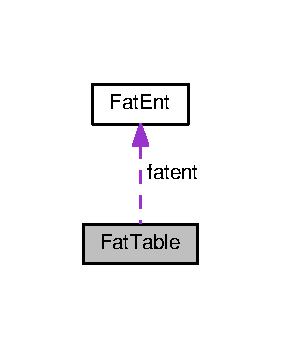
\includegraphics[width=136pt]{classFatTable__coll__graph}
\end{center}
\end{figure}
\subsection*{Public Member Functions}
\begin{DoxyCompactItemize}
\item 
\hyperlink{classFatTable_a848a7e9e14bd9d24fcfb48449fdfae77}{Fat\+Table} ()
\begin{DoxyCompactList}\small\item\em class Fat\+Eent \end{DoxyCompactList}\item 
ui \hyperlink{classFatTable_ae5bcce7262ced6cab5a164c40307c350}{insert} (const char $\ast$name, const ui \&size)\hypertarget{classFatTable_ae5bcce7262ced6cab5a164c40307c350}{}\label{classFatTable_ae5bcce7262ced6cab5a164c40307c350}

\begin{DoxyCompactList}\small\item\em fatent.\+resize(0);\} \end{DoxyCompactList}\item 
bool {\bfseries g\+\_\+full} ()\hypertarget{classFatTable_a0cbc50b29715a3b78322072dc5e18138}{}\label{classFatTable_a0cbc50b29715a3b78322072dc5e18138}

\item 
vector$<$ ui $>$ \hyperlink{classFatTable_a566150049a050b7add0046800995bf06}{alloc\+\_\+space} (const string \&, ui)
\item 
bool \hyperlink{classFatTable_a1e1637f54b2cc7a6c436a3c8dd86f990}{free\+\_\+space} (const string \&)
\item 
ui {\bfseries g\+\_\+unused} ()\hypertarget{classFatTable_a7b290d7cbffd8ee2fb1deb5c84188c0e}{}\label{classFatTable_a7b290d7cbffd8ee2fb1deb5c84188c0e}

\item 
vector$<$ ui $>$ \hyperlink{classFatTable_a81b335ad0538ee26afd7db168516ab08}{clusters\+\_\+file} (const string \&)
\item 
vector$<$ ui $>$ \hyperlink{classFatTable_a30f820bb48f85776482ac5248735fdd2}{g\+\_\+clusters\+\_\+list} (const string \&)
\item 
void \hyperlink{classFatTable_a45b8a123cf7f9124a950aa27d9aa9e28}{show} ()
\end{DoxyCompactItemize}
\subsection*{Public Attributes}
\begin{DoxyCompactItemize}
\item 
vector$<$ \hyperlink{classFatlist}{Fatlist} $>$ {\bfseries fatlist}\hypertarget{classFatTable_aa6ba21e5bfde8f742c4fe3f181a44aa2}{}\label{classFatTable_aa6ba21e5bfde8f742c4fe3f181a44aa2}

\item 
\hyperlink{classFatEnt}{Fat\+Ent} {\bfseries fatent} \mbox{[}750\mbox{]}\hypertarget{classFatTable_a23728b70a23aa0f3311837e04159220e}{}\label{classFatTable_a23728b70a23aa0f3311837e04159220e}

\end{DoxyCompactItemize}


\subsection{Constructor \& Destructor Documentation}
\index{Fat\+Table@{Fat\+Table}!Fat\+Table@{Fat\+Table}}
\index{Fat\+Table@{Fat\+Table}!Fat\+Table@{Fat\+Table}}
\subsubsection[{\texorpdfstring{Fat\+Table()}{FatTable()}}]{\setlength{\rightskip}{0pt plus 5cm}Fat\+Table\+::\+Fat\+Table (
\begin{DoxyParamCaption}
{}
\end{DoxyParamCaption}
)}\hypertarget{classFatTable_a848a7e9e14bd9d24fcfb48449fdfae77}{}\label{classFatTable_a848a7e9e14bd9d24fcfb48449fdfae77}


class Fat\+Eent 

class \hyperlink{classFatTable}{Fat\+Table} , fatent(0)\{

C\+AN\textquotesingle{}T BE \textquotesingle{}0\textquotesingle{} 

\subsection{Member Function Documentation}
\index{Fat\+Table@{Fat\+Table}!alloc\+\_\+space@{alloc\+\_\+space}}
\index{alloc\+\_\+space@{alloc\+\_\+space}!Fat\+Table@{Fat\+Table}}
\subsubsection[{\texorpdfstring{alloc\+\_\+space(const string \&, ui)}{alloc_space(const string &, ui)}}]{\setlength{\rightskip}{0pt plus 5cm}vector$<$ ui $>$ Fat\+Table\+::alloc\+\_\+space (
\begin{DoxyParamCaption}
\item[{const string \&}]{file, }
\item[{ui}]{size}
\end{DoxyParamCaption}
)}\hypertarget{classFatTable_a566150049a050b7add0046800995bf06}{}\label{classFatTable_a566150049a050b7add0046800995bf06}
Pega o nº do cluster necessarios

Checa para ver se ainda cabe nos clusters restantes.

Encontra o cluster adequado para a primeira posicao. C\+Luster encontrado.

Checa se existe arquivo de mesmo nome. Se sim, R\+E\+T\+U\+RN.

Nao tem espaço para reaproveitar no vetor de nomes.

Reaproveita o espaço e

remove esse espaço dos livres para reuso.

Lista contendo os cluter ussados

Arquivo vazio ou com tam $<$ \hyperlink{classQtt}{Qtt} \+:\+: C\+L\+U\+S\+T\+ER

Lista de posicoes do cluster do arquivo recebido

used = true, eof = true, next = -\/1 (valor qqer)

Parametros sao as posicoes do cluster predecessor.

Proximo cilindro alocado para insercao.

assert(qtt $>$= 2)

Inserir o resto do arquivo.

Inserir o ultimo setor; calcular também seu tamanho exato


\begin{DoxyItemize}
\item 
\end{DoxyItemize}

used = true, eof = false, next = -\/1

Todo os clusters na tsbela fat adequadamente enumerados \index{Fat\+Table@{Fat\+Table}!clusters\+\_\+file@{clusters\+\_\+file}}
\index{clusters\+\_\+file@{clusters\+\_\+file}!Fat\+Table@{Fat\+Table}}
\subsubsection[{\texorpdfstring{clusters\+\_\+file(const string \&)}{clusters_file(const string &)}}]{\setlength{\rightskip}{0pt plus 5cm}vector$<$ ui $>$ Fat\+Table\+::clusters\+\_\+file (
\begin{DoxyParamCaption}
\item[{const string \&}]{file}
\end{DoxyParamCaption}
)}\hypertarget{classFatTable_a81b335ad0538ee26afd7db168516ab08}{}\label{classFatTable_a81b335ad0538ee26afd7db168516ab08}
Encontrou o arquivo \index{Fat\+Table@{Fat\+Table}!free\+\_\+space@{free\+\_\+space}}
\index{free\+\_\+space@{free\+\_\+space}!Fat\+Table@{Fat\+Table}}
\subsubsection[{\texorpdfstring{free\+\_\+space(const string \&)}{free_space(const string &)}}]{\setlength{\rightskip}{0pt plus 5cm}bool Fat\+Table\+::free\+\_\+space (
\begin{DoxyParamCaption}
\item[{const string \&}]{get\+\_\+out}
\end{DoxyParamCaption}
)}\hypertarget{classFatTable_a1e1637f54b2cc7a6c436a3c8dd86f990}{}\label{classFatTable_a1e1637f54b2cc7a6c436a3c8dd86f990}
Reseta objeto; pra poder usar novamente

getchar();

Para representar

\hyperlink{classCluster}{Cluster} livre para reuso

\hyperlink{classCluster}{Cluster} livre novamente \+:) \index{Fat\+Table@{Fat\+Table}!g\+\_\+clusters\+\_\+list@{g\+\_\+clusters\+\_\+list}}
\index{g\+\_\+clusters\+\_\+list@{g\+\_\+clusters\+\_\+list}!Fat\+Table@{Fat\+Table}}
\subsubsection[{\texorpdfstring{g\+\_\+clusters\+\_\+list(const string \&)}{g_clusters_list(const string &)}}]{\setlength{\rightskip}{0pt plus 5cm}vector$<$ ui $>$ Fat\+Table\+::g\+\_\+clusters\+\_\+list (
\begin{DoxyParamCaption}
\item[{const string \&}]{file}
\end{DoxyParamCaption}
)}\hypertarget{classFatTable_a30f820bb48f85776482ac5248735fdd2}{}\label{classFatTable_a30f820bb48f85776482ac5248735fdd2}
cout $<$$<$ \char`\"{}\+Buscando por \+:: \char`\"{} $<$$<$ file $<$$<$ endl;

Caso especial de arquivo com apenas um cluster \index{Fat\+Table@{Fat\+Table}!show@{show}}
\index{show@{show}!Fat\+Table@{Fat\+Table}}
\subsubsection[{\texorpdfstring{show()}{show()}}]{\setlength{\rightskip}{0pt plus 5cm}void Fat\+Table\+::show (
\begin{DoxyParamCaption}
{}
\end{DoxyParamCaption}
)}\hypertarget{classFatTable_a45b8a123cf7f9124a950aa27d9aa9e28}{}\label{classFatTable_a45b8a123cf7f9124a950aa27d9aa9e28}
Para depois imprimir os setores \+:/

Calcula os setores a serem mostrados. 

The documentation for this class was generated from the following files\+:\begin{DoxyCompactItemize}
\item 
estruturas.\+hpp\item 
estruturas.\+cpp\end{DoxyCompactItemize}

\hypertarget{classHardDrive}{}\section{Hard\+Drive Class Reference}
\label{classHardDrive}\index{Hard\+Drive@{Hard\+Drive}}
\subsection*{Public Member Functions}
\begin{DoxyCompactItemize}
\item 
\hyperlink{classCylinder}{Cylinder} {\bfseries g\+\_\+cylinder} (const ui \&i)\hypertarget{classHardDrive_abc9084285a1cf0576596db2d9ef0c99b}{}\label{classHardDrive_abc9084285a1cf0576596db2d9ef0c99b}

\item 
bool {\bfseries g\+\_\+full} ()\hypertarget{classHardDrive_a40c97bea8fb3073d24fddf2d88ab1d38}{}\label{classHardDrive_a40c97bea8fb3073d24fddf2d88ab1d38}

\item 
ui \hyperlink{classHardDrive_abe41cc759c1ef69c3588cac961a13bed}{insert\+\_\+file} ()\hypertarget{classHardDrive_abe41cc759c1ef69c3588cac961a13bed}{}\label{classHardDrive_abe41cc759c1ef69c3588cac961a13bed}

\begin{DoxyCompactList}\small\item\em public \end{DoxyCompactList}\item 
bool \hyperlink{classHardDrive_a029807e52c15e36d3daabf18a5518f11}{remove\+\_\+file} ()\hypertarget{classHardDrive_a029807e52c15e36d3daabf18a5518f11}{}\label{classHardDrive_a029807e52c15e36d3daabf18a5518f11}

\begin{DoxyCompactList}\small\item\em Funcao Q\+UE I\+N\+T\+E\+R\+E\+S\+SA ao usuario que vai gusrdar um arquivo. \end{DoxyCompactList}\item 
void {\bfseries show\+\_\+file} ()\hypertarget{classHardDrive_a950c4bdeb4f2e6b312d8c543e605830f}{}\label{classHardDrive_a950c4bdeb4f2e6b312d8c543e605830f}

\item 
void {\bfseries show\+\_\+\+F\+AT} ()\hypertarget{classHardDrive_a504d5ac923ed97b3400cb96e721c1f00}{}\label{classHardDrive_a504d5ac923ed97b3400cb96e721c1f00}

\end{DoxyCompactItemize}
\subsection*{Static Public Member Functions}
\begin{DoxyCompactItemize}
\item 
static const ui {\bfseries g\+\_\+n\+\_\+cylinders} ()\hypertarget{classHardDrive_a62d430a815c360dbcc2b80c8da2d7ffe}{}\label{classHardDrive_a62d430a815c360dbcc2b80c8da2d7ffe}

\item 
static constexpr ui {\bfseries g\+\_\+\+C\+L\+U\+S\+T\+E\+RS} ()\hypertarget{classHardDrive_aac2e81c55187c2fae1784c1cefe8bb85}{}\label{classHardDrive_aac2e81c55187c2fae1784c1cefe8bb85}

\end{DoxyCompactItemize}


The documentation for this class was generated from the following files\+:\begin{DoxyCompactItemize}
\item 
estruturas.\+hpp\item 
estruturas.\+cpp\end{DoxyCompactItemize}

\hypertarget{classQtt}{}\section{Qtt Class Reference}
\label{classQtt}\index{Qtt@{Qtt}}
\subsection*{Static Public Attributes}
\begin{DoxyCompactItemize}
\item 
static constexpr ui {\bfseries S\+E\+C\+T\+OR} = 512\hypertarget{classQtt_a177e5a4df6a1fa166aacd96ff690280c}{}\label{classQtt_a177e5a4df6a1fa166aacd96ff690280c}

\item 
static constexpr ui {\bfseries C\+L\+U\+S\+T\+ER} = 4 $\ast$ S\+E\+C\+T\+OR\hypertarget{classQtt_a2a7a98fbf047bb63bd55678f8633ab94}{}\label{classQtt_a2a7a98fbf047bb63bd55678f8633ab94}

\item 
static constexpr ui {\bfseries T\+R\+A\+CK} = 15 $\ast$ C\+L\+U\+S\+T\+ER\hypertarget{classQtt_af3bc3ac1337b451d2874b25ab097e099}{}\label{classQtt_af3bc3ac1337b451d2874b25ab097e099}

\item 
static constexpr ui {\bfseries C\+Y\+L\+I\+N\+D\+ER} = 5 $\ast$ T\+R\+A\+CK\hypertarget{classQtt_a978f12a5bb314b193446ea6f64edad85}{}\label{classQtt_a978f12a5bb314b193446ea6f64edad85}

\item 
static constexpr ui {\bfseries H\+A\+R\+D\+D\+R\+I\+VE} = 10 $\ast$ C\+Y\+L\+I\+N\+D\+ER\hypertarget{classQtt_ac85fa07393a2f59111cf9f45d4c05f0b}{}\label{classQtt_ac85fa07393a2f59111cf9f45d4c05f0b}

\end{DoxyCompactItemize}


The documentation for this class was generated from the following file\+:\begin{DoxyCompactItemize}
\item 
estruturas.\+hpp\end{DoxyCompactItemize}

\hypertarget{classSector}{}\section{Sector Class Reference}
\label{classSector}\index{Sector@{Sector}}


Unidades basicas de armazenamento (num HD orientado a setores)  




{\ttfamily \#include $<$estruturas.\+hpp$>$}

\subsection*{Public Member Functions}
\begin{DoxyCompactItemize}
\item 
\hyperlink{classSector_acba0ffc50e70c7b4dac61a190d26b019}{Sector} ()\hypertarget{classSector_acba0ffc50e70c7b4dac61a190d26b019}{}\label{classSector_acba0ffc50e70c7b4dac61a190d26b019}

\begin{DoxyCompactList}\small\item\em \mbox{[}512\mbox{]}; \end{DoxyCompactList}\item 
const char $\ast$ {\bfseries g\+\_\+byte\+\_\+s} ()\hypertarget{classSector_ab5d1a8835ec6b6ca219747f792079748}{}\label{classSector_ab5d1a8835ec6b6ca219747f792079748}

\item 
bool {\bfseries g\+\_\+eof} ()\hypertarget{classSector_a0de4324c638872ff7f81899257883fe7}{}\label{classSector_a0de4324c638872ff7f81899257883fe7}

\item 
int {\bfseries g\+\_\+last\+\_\+valid} ()\hypertarget{classSector_aaa5f0478cd5e73cf792a98c73772e0ec}{}\label{classSector_aaa5f0478cd5e73cf792a98c73772e0ec}

\item 
ui {\bfseries insert\+\_\+last} (const string \&, const ui \&, int)\hypertarget{classSector_a3de8da2bad055e2b4cd3d665633053b6}{}\label{classSector_a3de8da2bad055e2b4cd3d665633053b6}

\item 
ui \hyperlink{classSector_a934dc752fbfb2b98075c500904b2ca6b}{insert} (const char $\ast$, const ui \&, const ui \&, string)
\begin{DoxyCompactList}\small\item\em cluster, posicao do setor, last valid position \end{DoxyCompactList}\end{DoxyCompactItemize}


\subsection{Detailed Description}
Unidades basicas de armazenamento (num HD orientado a setores) 

\subsection{Member Function Documentation}
\index{Sector@{Sector}!insert@{insert}}
\index{insert@{insert}!Sector@{Sector}}
\subsubsection[{\texorpdfstring{insert(const char $\ast$, const ui \&, const ui \&, string)}{insert(const char *, const ui &, const ui &, string)}}]{\setlength{\rightskip}{0pt plus 5cm}ui Sector\+::insert (
\begin{DoxyParamCaption}
\item[{const char $\ast$}]{cluster, }
\item[{const ui \&}]{next, }
\item[{const ui \&}]{pos, }
\item[{string}]{op = {\ttfamily string(\char`\"{}\char`\"{})}}
\end{DoxyParamCaption}
)}\hypertarget{classSector_a934dc752fbfb2b98075c500904b2ca6b}{}\label{classSector_a934dc752fbfb2b98075c500904b2ca6b}


cluster, posicao do setor, last valid position 

class \hyperlink{classSector}{Sector}

private public pos == 0,1,2,3 (nº do setor NO cluster) \begin{DoxyVerb}CAGUEI! Sa porra fica dando SEMPRE this->used == 1. Como?!?!
\end{DoxyVerb}
 / if(this-\/$>$used $>$ 0)\{cout$<$$<$ this-\/$>$used $<$$<$ \char`\"{} Erro\+: sobreposicao de setores\textbackslash{}n\char`\"{};throw 1.\+1;\}

Ou seja, todos os bytes do setor sao utilizados 

The documentation for this class was generated from the following files\+:\begin{DoxyCompactItemize}
\item 
estruturas.\+hpp\item 
estruturas.\+cpp\end{DoxyCompactItemize}

\hypertarget{classTime}{}\section{Time Class Reference}
\label{classTime}\index{Time@{Time}}


Final das Estruturas basicas.  




{\ttfamily \#include $<$estruturas.\+hpp$>$}

\subsection*{Static Public Attributes}
\begin{DoxyCompactItemize}
\item 
static const int {\bfseries S\+E\+E\+K\+\_\+\+M\+E\+AN} = 4\hypertarget{classTime_a3977bad6b54ae3a1600d73060251e22f}{}\label{classTime_a3977bad6b54ae3a1600d73060251e22f}

\item 
static const int {\bfseries S\+E\+E\+K\+\_\+\+M\+IN} = 1\hypertarget{classTime_a4d62bba8f4c6647a754aa164298d867c}{}\label{classTime_a4d62bba8f4c6647a754aa164298d867c}

\item 
static const int {\bfseries L\+A\+T\+E\+N\+C\+Y\+\_\+\+M\+E\+AN} = 6\hypertarget{classTime_a2e49c1935993babc40df360de53664b2}{}\label{classTime_a2e49c1935993babc40df360de53664b2}

\item 
static const int {\bfseries T\+R\+A\+N\+S\+F\+E\+R\+\_\+\+T\+R\+A\+CK} = 12\hypertarget{classTime_a6780787c8246709d2c43567915262518}{}\label{classTime_a6780787c8246709d2c43567915262518}

\item 
static constexpr double {\bfseries T\+R\+A\+N\+S\+F\+E\+R\+\_\+\+C\+L\+U\+S\+T\+ER} = T\+R\+A\+N\+S\+F\+E\+R\+\_\+\+T\+R\+A\+CK/15.\+0\hypertarget{classTime_a96badaf914d28009d79858081b049d6f}{}\label{classTime_a96badaf914d28009d79858081b049d6f}

\end{DoxyCompactItemize}


\subsection{Detailed Description}
Final das Estruturas basicas. 

The documentation for this class was generated from the following file\+:\begin{DoxyCompactItemize}
\item 
estruturas.\+hpp\end{DoxyCompactItemize}

\hypertarget{classTrack}{}\section{Track Class Reference}
\label{classTrack}\index{Track@{Track}}
\subsection*{Public Member Functions}
\begin{DoxyCompactItemize}
\item 
\hyperlink{classCluster}{Cluster} {\bfseries g\+\_\+cluster} (const ui \&i) const \hypertarget{classTrack_a1b68a43b28d8c26d7af01a9a8e8c1ddf}{}\label{classTrack_a1b68a43b28d8c26d7af01a9a8e8c1ddf}

\item 
vector$<$ \hyperlink{classCluster}{Cluster} $>$ {\bfseries g\+\_\+clusters} () const \hypertarget{classTrack_ad84a7049f08ce72e64d6183b9e41c6f4}{}\label{classTrack_ad84a7049f08ce72e64d6183b9e41c6f4}

\item 
bool {\bfseries g\+\_\+full} ()\hypertarget{classTrack_ad93cf5c10d7170353b0476216857c3ce}{}\label{classTrack_ad93cf5c10d7170353b0476216857c3ce}

\item 
bool \hyperlink{classTrack_a84b7957f08de9ffe8c53fb7050f38cdd}{s\+\_\+full} ()
\begin{DoxyCompactList}\small\item\em public \end{DoxyCompactList}\item 
ui \hyperlink{classTrack_a9c119d10ee46f6e00fd37425b78d1a43}{insert} (const char $\ast$, ui, const ui \&, string)\hypertarget{classTrack_a9c119d10ee46f6e00fd37425b78d1a43}{}\label{classTrack_a9c119d10ee46f6e00fd37425b78d1a43}

\begin{DoxyCompactList}\small\item\em Retorna o numero do novo cluster ocupado. \end{DoxyCompactList}\item 
char $\ast$ {\bfseries g\+\_\+cluster\+\_\+content} (ui)\hypertarget{classTrack_a95108a0e25c400c8d073c41c1af147c2}{}\label{classTrack_a95108a0e25c400c8d073c41c1af147c2}

\end{DoxyCompactItemize}
\subsection*{Static Public Member Functions}
\begin{DoxyCompactItemize}
\item 
static constexpr ui {\bfseries g\+\_\+\+C\+L\+U\+S\+T\+E\+RS} ()\hypertarget{classTrack_a116fdaace82b411f98b16a7c5e1b91b1}{}\label{classTrack_a116fdaace82b411f98b16a7c5e1b91b1}

\end{DoxyCompactItemize}


\subsection{Member Function Documentation}
\index{Track@{Track}!s\+\_\+full@{s\+\_\+full}}
\index{s\+\_\+full@{s\+\_\+full}!Track@{Track}}
\subsubsection[{\texorpdfstring{s\+\_\+full()}{s_full()}}]{\setlength{\rightskip}{0pt plus 5cm}bool Track\+::s\+\_\+full (
\begin{DoxyParamCaption}
{}
\end{DoxyParamCaption}
)}\hypertarget{classTrack_a84b7957f08de9ffe8c53fb7050f38cdd}{}\label{classTrack_a84b7957f08de9ffe8c53fb7050f38cdd}


public 

class \hyperlink{classTrack}{Track} private 

The documentation for this class was generated from the following files\+:\begin{DoxyCompactItemize}
\item 
estruturas.\+hpp\item 
estruturas.\+cpp\end{DoxyCompactItemize}

%--- End generated contents ---

% Index
\backmatter
\newpage
\phantomsection
\clearemptydoublepage
\addcontentsline{toc}{chapter}{Index}
\printindex

\end{document}
